\documentclass[article,shortnames]{jss}

%%%%%%%%%%%%%%%%%%%%%%%%%%%%%%
%% declarations for jss.cls %%%%%%%%%%%%%%%%%%%%%%%%%%%%%%%%%%%%%%%%%%
%%%%%%%%%%%%%%%%%%%%%%%%%%%%%%
\usepackage{amsmath}                
\usepackage{amssymb}
\usepackage{amsthm}

%% almost as usual
\author{Daniel Conn\\ UCLA SPH, Biostatistics \AND Tuck Ngun\\Department of Human Genetics David Geffen School of Medicine, UCLA \AND  Gang Li\\UCLA SPH, Biostatistics \And Christina M. Ramirez\\UCLA SPH, Biostatistics}
\title{Fuzzy Forests: A New WGCNA Based Random Forest Algorithm for Correlated, High-Dimensional Data}

%% for pretty printing and a nice hypersummary also set:
\Plainauthor{Daniel Conn, Christina Ramirez} %% comma-separated
\Plaintitle{Fuzzy Forests: A New WGCNA Based Random Forest Algorithm for High-Dimensional, Correlated Data} %% without formatting
\Shorttitle{\pkg{fuzzyforest}: Fuzzy Forests in \proglang{R}} %% a short title (if necessary)

%% an abstract and keywords
\Abstract{In this paper we introduce fuzzy forests, a new machine learning algorithm for ranking the importance of features in high-dimensional classification and regression
 problems.  Fuzzy forests is specifically designed to provide unbiased rankings of variable importance in the presence of correlated features. 
Fuzzy forests uses Weighted Gene Coexpressionn Network Analysis (WGCNA) to detect groups of highly correlated features.  Unbiased rankings are
obtained by fitting separate random forests on each module.  We also introduce our implementation of fuzzy forests in the \proglang{R} package, \pkg{fuzzyforests}.}
\Keywords{Random Forests, WGCNA, machine learning,\proglang{R}}
\Plainkeywords{Random Forests, WGCNA, machine learning,R} %% without formatting
%% at least one keyword must be supplied

%% publication information
%% NOTE: Typically, this can be left commented and will be filled out by the technical editor
%% \Volume{50}
%% \Issue{9}
%% \Month{June}
%% \Year{2012}
%% \Submitdate{2012-06-04}
%% \Acceptdate{2012-06-04}

%% The address of (at least) one author should be given
%% in the following format:
\Address{
  Daniel Conn\\
  Department of Biostatistics\\
  UCLA School of Public Health\\
  Los Angeles, United States of America\\
  E-mail: \email{djconn17@gmail.com}\\
}
%% It is also possible to add a telephone and fax number
%% before the e-mail in the following format:
%% Telephone: +43/512/507-7103
%% Fax: +43/512/507-2851

%% for those who use Sweave please include the following line (with % symbols):
%% need no \usepackage{Sweave.sty}

%% end of declarations %%%%%%%%%%%%%%%%%%%%%%%%%%%%%%%%%%%%%%%%%%%%%%%


\begin{document}

%% include your article here, just as usual
%% Note that you should use the \pkg{}, \proglang{} and \code{} commands.

\section{Introduction}
%% Note: If there is markup in \(sub)section, then it has to be escape as above.
The problem of identifying important features in the presence of correlation has been an area of intense research within the statistics
and machine learning community.  Biological applications have, in particular, spurred the development of high dimensional feature selection methods.   
While model based feature selection algorithms such as the LASSO or SCAD may efficiently detect important features in presence of correlation \citep{raskutti2010restricted}, this efficiency comes at the cost of making parametric assumptions that may not hold in practice. 
 
Random forest variable importance measures (VIMs) offer a nonparametric alternative to model based feature selection algorithms \citep{breiman2001random}.
Random forests is a popular ensemble based machine learning algorithm.  While random forest VIMs have demonstrated the ability to accurately capture the true 
importance of features in settings where the features are independent, it is well-known that random forests VIMs are biased when features are correlated
with one another (\citep{strobl2007bias}; \citep{strobl2008conditional}; \citep{nicodemus2009predictor}).

Fuzzy forests cope with correlated features by taking a piecewise approach.  We partition the set of features into distinct modules such that the correlation within each module is high and the correlation between modules is low.  We then use an iterative feature selection algorithm as in \citep{diaz2006gene} to select the most important
features from each module.  A random forest is then fit to the features that have survived this first round.  A final iterative random forest,  combining features from all
modules, selects the top $k$ features. 

There are a variety of algorithms for partitioning features into distinct, high correlation modules.  In this regard, WGCNA is our method of choice.  WGCNA is a rigorous framework for detecting correlation networks \citep{zhang2005general}.  Although it was first developed to detect modules of highly correlated genes, it has found application in a variety of biological contexts.  The \proglang{R} package \pkg{WGCNA} is a robust, computationally efficient, and well-documented implementation of the WGCNA framework.  We expect that researchers already familiar with \pkg{WGCNA} will easily adopt the fuzzy forests algorithm and we expect that newcomers to WGCNA will be able to make good use of \pkg{WGCNA}'s fine documentation and tutorials.
              
The article is organized as follows.  In section 2 of this article, we briefly review the random forests, WGCNA, and introduce the fuzzy forests algorithm.
In section 3, we introduce the \proglang{R} package \pkg{fuzzyforest}.  In section 4, we conduct simulations comparing fuzzy forests to random forests.  In section 5, we use fuzzy forests to determine which biological factors are important in determining how well an HIV patient copes with the virus.  Section 6 ends the article with a discussion and summary of our results. 

\section{Variable Importance Measures and the Fuzzy Forests Algorithm}
\subsection{Variable Importance Measures}[2.1]
In this section, we introduce basic notation and define variable importance measures.  We assume that our data comes in the form of $n$ independently and identically distributed iid
pairs $(X,Y) \sim G$.  Here $X$ is a $p$ dimensional feature vector and $Y$ is a scalar outcome.  The value of the $v$th feature for the $i$th subject will be denoted by $X_{i}^{(v)}$.
The feature vector for the $i$th subject is denoted by $X_{i}=(X_{i}^{(1)},\ldots,X_{i}^{(p)})$.   Finally, let $X^{(v)}=(X_{1}^{(v)},\ldots,X_{n}^{(v)})$ be the set of values for feature $v$ across
all $n$ subjects.

In the case of both classification and regression we are interested in modeling the conditional mean of $Y$ given a feature vector $X_{i}$.  We denote this conditional mean alternatively as $E[Y|X]$ or $f(X)$.
In the case of regression, we assume that $Y|X$ has distribution $f(X) + \epsilon$, where the $\epsilon$ are $iid$ with variance $\sigma^{2}$.   In the regression setting, $Y$ is unrestricted. 
In classification, $Y$ is restricted to take the value 0 or 1 and $Y|X$ is a Bernoulli trial with mean $E[Y|X]$.  

If the goal is to predict a new outcome $Y$ based off of measurements, $X$, a good estimate of $f(X)$ is all that is required.
We are interested in more than prediction.  We are interested in understanding how $f(X)$ changes as function of particular features. 
If the value of $f(X)$ varies widely according to a particular value of the $v$th feature, $X^{(v)}$ is, in some sense, an ``important" determinant of
the outcome, $Y$.  

If $p$ is low dimensional $(p=1,2)$, we can simply plot our estimate of $f(X)$ to understand how it varies as function of $X$. 
If $p$ is moderate or large, $f(X)$ is difficult to interpret.  It is most common in this case, to assume $f(X)$ has a specific parametric
form so that $f_{\beta}(X)$ is known up to a finite dimensional parameter $\beta$.  In the case of linear regression, $\beta$ is a vector of
regression coefficients and we can measure the importance of one feature versus another feature by examining the absolute magnitude 
of their corresponding coefficents.    

If the parametric model $f_{\beta}(X)$ is a close approximation to $f(X)$, it is possible that interpretations based off of $\hat{f}_{\hat{\beta}}(X)$
will not be misleading.  Likewise, if $f_{\beta}(X)$ is a poor approximation of $f(X)$, the resulting interpretation will be misleading.  
The parametric approximation $f_{\beta}(X)$ may be inadequate for a variety of reasons.  This may occur if important features are 
not observed.  Even if all appropriate features are measured, $f_{\beta}(X)$ may fail to capture important interactions between features.
If $f_{\beta}(X)$ is a linear regression model, $\sum_{v=1}^{p}\beta_{v}X^{(v)}$, the true $f(X)$ may be nonlinear in such a way that this best linear approximation fails to capture.
  
Permutation VIMs provide a means of summarizing the importance of individual features without making parametric assumptions.
In the case of regression, we define the permutation VIM of feature $v$, $X^{(v)}$, as 
\begin{equation}
VIM(v)=E(f(X^{(1)}_{i},\ldots,X^{(v)}_{i},\ldots,X^{(p)}_{i}) - f(X^{(1)}_{i},\ldots,\tilde{X}^{(v)}_{i},\ldots,X^{(p)}_{i}))^{2}.
\end{equation}
Here, $X^{(v)}_{i}$ and $\tilde{X}^{(v)}_{i}$ are iid with distribution $G_{X^{(v)}}$ where $G_{X^{(v)}}$ is the marginal distribution of $X^{(v)}_{i}$.  This form of the VIM
is given in a slightly different form in \cite{gregorutti2013correlation} and \cite{zhu2012reinforcement}.
\cite{gregorutti2013correlation} present a similar expression for the case of classification.  
These authors also discuss conditions under which the estimate of the permutation VIM derived from random forests is consistent. 

         
\subsection{An Introduction to Random Forests}[2.2]
Random forests is a popular ensemble method that has been applied in the setting of both classification and regression.  The random forests algorithm works
by combining the predictions of an ensemble of classification and regression trees.  Each tree is grown on a separate bootstrap sample of the data.  The number
of trees grown in this manner is denoted as $ntree$.  The subjects that are not selected in a particular bootstrap sample are said to be ``out of bag."  

Call the $k$th tree $\hat{f}_{k}(X)$.  In the case of regression trees,
$\hat{f}(X)=\frac{1}{ntree}\sum_{k=1}^{ntree}\hat{f}_{k}(X)$.  In the case of classification, $\hat{f}(X)$ is the majority vote of the $ntree$ predictions given
by $\hat{f}_{k}(X)$.  Each regression tree is highly unstable and gives highly variable predictions.  Averaging multiple trees over
many bootstrap samples leads to more stable estimates of $f(X)$.  The algorithm described thus far is known as bagging (bootstrap-aggregating).  This 
algorithm is a special case of random forests.  

A further element of randomness is introduced by random forests.  Before a node in a particular tree is split, a subset of features is chosen at random.  Of these randomly 
chosen features, the feature with the highest marginal importance is used to split the node.  The number of randomly selected features at each stage is
commonly denoted as $mtry$.  High values of $mtry$ tend to lead to just a few important features getting selected at the majority cut-points.
Lower values of $mtry$ allow more features to play a role in the estimation $f(X)$.  In the case of regression, a common default value of $mtry$ is $\sqrt{p}$.
In the case of classification  $\left\lfloor p/3 \right\rfloor$ is common choice.
  
Random forest VIMs are obtained by testing how predictive accuracy suffers when the values of individual predictors are permuted.  Let $OOB_{k} \subset \{1,\ldots, n\}$ 
be the out of bag samples in the $k$th bootstrap sample.  Let $\pi_{k}$ be a random permutation of the elements of $OOB_{k}$ and let   
$\pi_{k}^{(v)}(X_{i}) = (X_{i}^{(1)},\ldots,X_{\pi_{k}(i)}^{(v)},\ldots,X_{i}^{(p)}),$ where $i \in OOB_{k}$.   In other words, $\pi_{k}^{(v)}$ 
permutes the values of the $v$th feature across all out of bag subjects.  In the case of regression, the variable importance of the $i$th feature from the $k$th tree is defined as
\begin{equation}
\widehat{VIM}^{k}(v)= \frac{\sum_{i \in OOB_{k}}(y_{i}-\hat{f}^{k}(\pi_{k}^{(v)}(X_{i}))^{2} - (y_{i} - \hat{f}^{k}(X_{i}))^{2}}{|OOB_{k}|}
\end{equation}
The variable importance for the entire random forest is defined as
\begin{equation}
\widehat{VIM}(v) = \frac{\sum_{k=1}^{ntree}\widehat{VIM}^{k}(v)}{ntree}
\end{equation}

\subsection{A Brief Review of WGCNA}[2.3]
WGCNA is a rigorous framework for constructing a network of features. 
This network is then used to determine clusters or modules of inter-related features. 
We briefly review the steps of a WGCNA network analysis.  Our review closely follows that of \cite{zhang2005general}.  
The user first specifies a similarity function $s_{ij}=S(X^{(i)},X^{(j)})$ taking values between 0 and 1.  Both unsigned and signed 
networks are possible.  If the features are continuous, the most common choice of similarity function is $|Corr(X^{(i)},X^{(j)})|$ or 
$\frac{1 + Corr(X^{(i)},X^{(j)})}{2}$  according to whether the network is unsigned or signed \citep{zhang2005general}.

This similarity matrix is then transformed into an adjacency matrix $A=[a_{ij}]$.  This adjacency function determine how similarities translate
into properties of the network.  For example, in a hard-thresholded network, where nodes are either connected or unconnected,
the adjacency function determines how high the correlation has to be in order for two nodes to be connected.

This hard threshold function, denoted by $signum(s_{ij},\tau)$,  is the simplest choice of adjacency function.   
If $s_{ij} \geq \tau, a_{ij}=signum(s_{ij},\tau)=1$ otherwise $a_{ij}=0$.  Nodes are either connected or 
unconnected if the $signum$ adjacency function is used.  In practice, a soft-thresholded network is often more plausible than a 
hard-thresholded one.  The power function $a_{ij}=s_{ij}^{q}$ is common choice of soft-thresholding adjacency function.  Large values
of $q$ yield behavior closer to a hard-thresholded network.  Setting $q=1$ is equivalent to using the similarity function.
Once an adjacency function is calculated, a hierarchical clustering tree algorithm 
is used to define clusters of features.

It is common to apply this hierarchical clustering algorithm to the topological overlap matrix rather than the adjacency matrix.  The topological
overlap between two nodes is defined as 
\begin{equation}
\omega_{ij} = \frac{l_{ij} + a_{ij}}{min\{k_{i},k_{j}\} + 1 - a_{ij}}
\end{equation} 
where $l_{ij}=\sum_{u}a_{iu}a_{uj}$ and $k_{i}=\sum_{u}a_{iu}$\citep{horvath2011weighted}.  The topological overlap between two nodes can be high even if $a_{ij}$ is low.
This occurs when the two nodes are strongly connected to the same set of nodes.  Use of topological overlap rather
than the adjacencies may lead to more distinct modules\citep{zhang2005general}.

In many biological contexts, it is suspected that only a few features are highly connected.  This prior knowledge leads to the scale-free criterion for
determining which value of $q$ to select.  A network is said to have a generalized scale-free topology if $p(k) \sim k^{\gamma}$ or
 $\log_{10}(p(k)) \propto \log_{10}(k)$\citep{zhang2005general}.  This suggests that one should select a smaller value of $q$ such that the $R^{2}$ between 
  $\log_{10}(p(k))$ and $\log_{10}(k)$ is high.
  
\subsection{The Fuzzy Forests Algorithm}[2.4]
The fuzzy forests algorithm is an extension of random forests designed to obtain less biased variable importance rankings in the presence
of correlated features.  In following section, we describe the motivation behind fuzzy forests and explain why it
provides less biased estimates of VIMs.  In this section, we describe the algorithm.

The fuzzy forests algorithm can be subdivided into two steps: a screening step and a selection step.  The screening step works in a piecewise fashion
to screen out unimportant features.  The screening step takes as input a partition of the features such that the correlation within each partition is 
roughly constant.  Our package, \pkg{fuzzyforest}, facilitates the use of WGCNA to obtain such a partition of features.  However, 
it is possible to use alternative methods to partition the features.  Denote this partitioning of the features by set $P=\{P_{1},\ldots,P_{m}\}$.
Let $p_{l}=|P_{l}|$ so that $\sum_{l=1}^{m}p_{l}=p$.

The screening step operates independently on each partition.  For each element of the partition $P_{l}$, the screening step fits an iterative series of
random forests to eliminate features in backwards stepwise fashion.  Starting with all features in the partition $P_{l}$, a random forest is fit using all
features in $P_{l}$.  The least important features are then eliminated, call the reduced set of features after the first random forest $P_{l}^{(1)}$.  
For example, the features with VIM in bottom 25\% might be dropped at each step. 
A 2nd random forest is fit using features in $P_{l}^{(1)}$.  The least important features from this latest random forest are then eliminated leading a
further reduced set of features $P_{l}^{(2)} \subset P_{l}^{(1)} \subset P_{l}$.  Call the subset obtained after the $k$th iteration $P_{l}^{(k)}$ and let
$p^{(k)}_{l}=|P_{l}^{(k)}|$.
Features are eliminated in this manner until a user-specified 
stopping criteria is reached.  For example, features may be eliminated until 5\% of the original $P_{l}$ features remain.  

The user must specify a few tuning parameters at the screening step.  First of all, the user must specify how many features are to be dropped after 
each random forest is fit, we call this fraction the $drop\_fraction$.   The user must also specify a stopping criteria. 
In \pkg{fuzzyforest} the user specifies what percentage of the original $p_{l}$ features to retain.  This percentage will be called the $keep\_fraction$.  
The first time the number of features drops below $keep\_fraction*p_{l}$, the iterative series of random forests will stop and the top 
$\left\lfloor keep\_fraction*p_{l} \right\rfloor$ features will be selected.  More precisely, for the first iteration $k$ such that $p^{(k)}_{l}<keep\_fraction*p_{l}$, 
we retain the top $\left\lfloor keep\_fraction*p_{l} \right\rfloor$ features from $P_{l}^{(k-1)}$.         

For each random forest, $mtry$ and $ntree$ must appropriately selected.  Since the number features varies across random forests, $mtree$
and $ntree$ must be a function of the current number of features.   Suppose we at iteration $k$ and are about fit a random forest to obtain
$P_{l}^{(k+1)}\subset P_{l}^{(k)}$.  In the case of regression, \pkg{fuzzyforest} lets $mtry=\sqrt{p^{(k)}_{l}}mtry\_factor$.  For classification 
\pkg{fuzzyforest} sets $mtry=\left\lfloor p^{(k)}_{l}/3 \right\rfloor mtry\_factor$.  In both cases, $mtry\_factor$ must be pre-specified by the user
with a default of 1.  The parameter $ntree$ must be set high enough to be able to pick up the effects
of important variables, however if $ntree$ is set too high, the iterative series of random forests will take a long time to run.  The package \pkg{fuzzyforest} sets $ntree=max(min\_ntree,p^{(k)}_{l}*ntree\_factor)$.
   
The selection step consists of one last iterative series of random forests. This series of random forests is fit on all features that have
been selected at the screening step.  Note that a separate choice of $drop\_fraction$, $mtry\_factor$, $min\_tree$,
and $ntree\_factor$ may be used.  In the package \pkg{fuzzyforest}, $keep\_fraction$ is implicitly defined by user.  The user specifies 
how many features will selected by the selection step.  

\subsection{Motivation for Fuzzy Forests Algorithm}[2.5]

The selection step of fuzzy forests is motivated by the following observation concerning the theoretical properties of VIMs. 
Let $G_{P^{(l)}}$ denote the joint distribution of the features in partition $P^{(l)}$ and let $X^{P^{(l)}} \sim G_{P^{(l)}}$.
Suppose that $X^{P^{(i)}} \perp X^{P^{(j)}}$ for all $i\neq j$ and suppose that $f(X)=\sum_{j=1}^{m}f_{j}(X^{P^{(j)}})$.  If we fit
a random forest using only the features in $P^{(l)}$ we are no longer estimating $E[Y|X]=f(X)$, instead we are estimating
 $E[E[Y|X]|X^{(l)}]=E[f(X)|X^{P^{(l)}}]=\sum_{j=1}^{m}E[f_{j}(X^{P^{(j)}})|X^{P^{(l)}}]=f_{l}(X^{P^{(l)}}) + \sum_{j\neq l}^{m}E[f_{j}(X^{P^{(j)}})]$

Suppose feature $v$ is in partition $P^{(l)}$.  The variable importance obtained by fitting a random forest to only those features in  $P^{(l)}$
 is estimating the following quantity: 
 \begin{equation}
 VIM^{*}(v)=E(f_{l}(X^{(l_{1})}_{i},\ldots,X^{(v)}_{i},\ldots,X^{(l_{m})}_{i}) - f_{l}(X^{(l_{1})}_{i},\ldots,\tilde{X}^{(v)}_{i},\ldots,X^{(l_{m})}_{i}))^{2}.
 \end{equation}
 Here, $X_{i}^{l_{k}}$ is the $k$th element of partition $P^{(l)}$. As in equation (1), $X^{(v)}$ and $\tilde{X}^{(v)}$ are iid from $G_{X^{(v)}}$.
 We see from this equation that $VIM^{*}(v)=VIM(v)$ if the true regression function is additive across modules and if the modules are independent
 of one another.  If our assumptions are met, the VIMs obtained by analyzing each module separately are asymptotically the same as those that 
would have been obtained if VIMs were obtained by analyzing all features at once.       

Therefore, the selection step of fuzzy forests achieves two goals.  First of all, it reduces the number of features that have to be 
analyzed at one time.  Second, the finite sample bias caused by correlated features is alleviated.  In 
\citep{nicodemus2009predictor}, it is observed that insignificant features that are correlated with a significant feature 
are more likely to be chosen at the root of tree than uncorrelated significant features.  The high importance of these insignificant
correlated features comes at the cost of the significant uncorrelated features.  When we analyze each module separately, features 
in different groups are no longer competing against one another.   

This above observations suggest that we should fit a separate random forest to each module and then report the the resulting
estimates of the VIMs.  Why does the fuzzy forests algorithm diverge from this simple procedure?
We stress that the VIMs obtained by analyzing each module separately are, in general, different than the VIMs obtained
by fitting a single random forests.  The assumptions of additivity across modules and independence of modules are quite strong.

The fuzzy forests algorithm relaxes these overly restrictive assumptions.  Fuzzy forests allows for interactions between features that
were found to be important within modules.  In biological applications, modules might represent different biological systems.
Thus, it is reasonable to allow these systems to interact with one another.  In fuzzy forests, the selection step acts as a screening mechanism.
Fuzzy forests is implicitly making the assumption that the features that have high VIMs within modules are also most likely to be the features
involved in interactions across modules.   

It is important that iterative random forests are used at the selection step.  When features from separate modules are combined,
the potential for bias due to correlation between features is re-introduced.  The iterative random forests, in practice, manage to
eliminate unimportant predictors which are correlated with important ones.  

We do not recommend interpreting the estimated VIMs too closely.  While the ranking of the VIMs obtained from
fuzzy forests are less biased than those derived from random forests, the estimated VIMs may still be quite biased.

\section{The fuzzyforest package}
The package \pkg{fuzzyforest}  has two functions for fitting the fuzzy forests model.  The first is \code{WGCNA_fuzzyforest}, the
second is \code{fuzzyforest}.  The function \code{WGCNA_fuzzyforest} automatically carries out a WGCNA analysis on the input features.
Then it uses the newly derived modules as input to the fuzzy forest algorithm.  The WGCNA analysis is carried out via the 
\code{blockwiseModules} function from the package \pkg{WGCNA}.  

The second function \code{fuzzyforest} assumes that the features have already been partitioned into separate modules.
In particular a user is able to carefully conduct a separate module detection analysis using \pkg{WGCNA}.  Such an 
analysis might find the smallest value of $p$ such that the scale-free topology criterion is met.  The function \code{fuzzyforest}
is then able to carry out the fuzzy forests algorithm using the output of \pkg{WGCNA}.

A number of tuning parameters must be specified before fuzzy forests can be run.   These tuning parameters are organized
into separate control objects.  Tuning parameters related to WGCNA are specified with an \code{S3} object of type \code{WGCNA_control}
with constructor \newline \code{WGCNA_control()}.
Similarly tuning parameters related to the screening step and the select step are specified through objects of type 
\code{screen_control} and \code{select_control}.  

We demonstrate the workings of \pkg{fuzzyforest} with a small simulation.
The features have multivariate normal distribution and were generated using the package \pkg{mvtnorm}.  
There are 5 modules.  Within each module the correlation between features
is .8 and the variance of each feature is 1.  The modules are independent of one another.
The true model is linear and two of the 5 modules have 2 significant coefficients set to 5.
\begin{CodeChunk}
\begin{CodeInput}
R> n <- 100
R> p <- 50
R> mod_sigma <- matrix(.8,10,10); diag(mod_sigma)=1
R> sigma <- as.matrix(.bdiag(lapply(1:5, function(j) mod_sigma))) 
R> X <- rmvnorm(n, mean=rep(0, 50), sigma=sigma)
R> beta <- c(rep(5,2),rep(0,10-2),rep(5,2),rep(0,50-12))
R> y <- X%*%beta + rnorm(n, sd=.1)
R> X <- as.data.frame(X)
R> fit <- WGCNA_fuzzyforest(X,y,WGCNA_params=WGCNA_control(minModuleSize=1)
+ ,screen_params = screen_control(keep_fraction=.5, drop_fraction=.2)
+ ,select_params = select_control(number_selected=4, drop_fraction=.1) 
+ ,num_processors=4)
\end{CodeInput}
\end{CodeChunk}
If the outcome, \code{y}, is a \code{factor} the random forests will be constructed using classification trees,
otherwise regression trees will be used. \code{WGCNA_fuzzyforest} returns an \code{S3} object of type 
\code{fuzzy_forest} consisting of a list.  This list contains a \code{data.frame} with the ranking and VIM 
of the selected features.  It also contains the final random forest that was fit at the selection step, along 
with the module membership and further information about the weighted co-expression network.

Objects of type \code{fuzzy_forest} have the usual generic methods.  The function \code{print} returns the list
of selected features.  The function \code{predict(fuzzy_forest, new_data)} takes in a \code{data.frame} or 
\code{matrix} and produces predictions via a random forest based on the selected features.  

The number of features selected by fuzzy forests must be pre-specified.  It is possible to fit separate models
selecting a different numbers of features for each model.  The predictive accuracy on a test set can then 
be used to select one of these models.  If a test set is unavailable a plot of the test error versus the number 
of features selected may shed light on when the fuzzy forests algorithm begins over-fitting.
Note that these models will not necessarily be nested.
  
The generic function \code{plot} yields a visual display of which modules are important.  The grey bars
represent what percentage of the total $p$ features fall into a particular module.  The blue bars represent
the percentage of selected features that fall into each module.  Applying the function \code{plot} to the
object \code{fit} above, we obtain the graph in figure 1.
\begin{figure}[hc]
\caption{Result of \code{plot(fit)}}
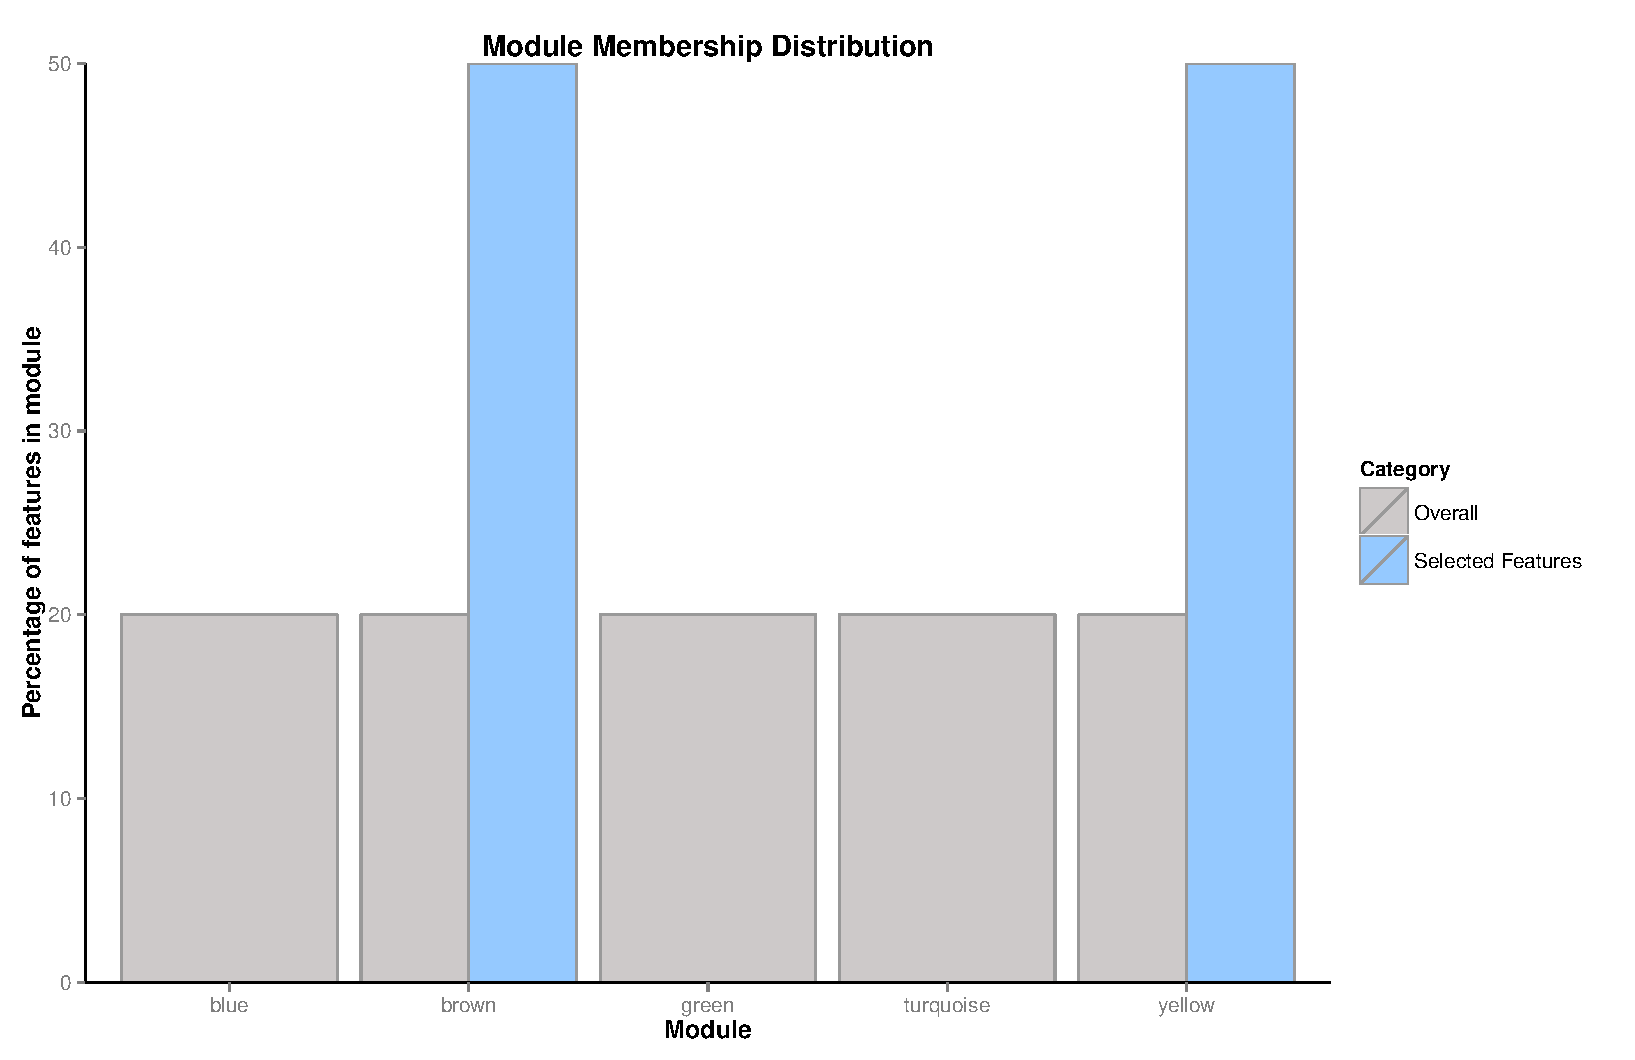
\includegraphics{ch3plot}
\end{figure}
\section{Simulations}
In this section we demonstrate the performance of fuzzy forests on a number of simulated data sets.
Our first set of simulations assumes a logistic regression model.  In all simulations, the sample size
was $n=1000$.  We let the number of features equal $p=100$ and $1000$.
For each simulation, we carried out 100 simulations.  In each simulation, the number of features selected
was 10.    

In the case, where $p=100$ there are 3 modules each of size 25.  The features were generated from a multivariate
normal distribution.  Each feature had variance 1.  The correlation within each module was 0.8.  The modules were independent of one 
another and there were an additional 25 features that were independent of each other and independent of each module.  

The true regression function is of the form $\log(p_{i}/(1-p_{i}))=X_{i}'\beta$ where $p_{i}$ is probability that
subject $i$ has outcome 1.   For the case when $p=100$,  the first 3 features are significant with values
1, .5, and .25.  The first 3 independent features are also significant with the same values.  We therefore have
\begin{equation}
\log(p_{i}/(1-p_{i})) = x_{1} + .5x_{2} + .25x_{3} + x_{76} + .5x_{77} + .25x_{78}
\end{equation}
where $x_{1}, x_{2}$ and $x_{3}$ are highly correlated and $ x_{76}, x_{77}$, and $x_{78}$ are independent.

We present below the results of fuzzy forests on 100 simulated data sets.  In addition to presenting the VIMs
for the significant predictors, we also present the VIMs for $x_{4}$ and $x_{79}$.  The simulation 
demonstrates fuzzy forests still has a tendency to select unimportant features that are correlated with important 
ones.   Although this bias is much reduced in comparison to random forests.
\begin{table}[hc]
\centering
\caption{Results of Simulation for $p=100$}
\begin{tabular}{lclcl}
Feature&Avg VIM& Probability of Selection\\
\hline
$x_{1}$  & .058 &  .75\\
$x_{2}$  & .023 &  .32\\
$x_{3}$  & .014 &  .21\\
$x_{4}$ & .007 &  .10\\
$x_{76}$ & .074 & 1.0\\
$x_{77}$ & .062 & .83 \\
$x_{78}$ & .001 & .14 \\
$x_{79}$ & .000 & 0.0
\end{tabular}
\end{table}

In the case where $p=1000$, there were 9 modules each of size 100.  Modules were independent of one
another and the correlation structure within modules was  once again .8.  The last 100 features were independent
of one another and of the 9 modules.  The first 3 of these independent features were significant yielding the following
regression function:
\begin{equation}
\log(p_{i}/(1-p_{i})) = x_{1} + .5x_{2} + .25x_{3} + x_{901} + .5x_{902} + .25x_{903}
\end{equation}
We show the average VIMs over 100 simulations and present the VIMs of $x_{4}$ and the $x_{904}$ in
addition to the significant ones. Note that the VIMs are at an overall lower level.  The selection probability 
of the most significant features remain somewhat similar to the case where $p=100$.  The selection 
probability of $x_{4}$ is lower than it was in the case of $p=100$, however, the selection probabilities
were overall lower in the simulation.
\begin{table}[hc]
\centering
\caption{Results of Simulation for $p=1000$}
\begin{tabular}{lclc|}
Feature & Avg VIM & Probability of Selection\\
\hline
$x_{1}$  & .023 & .70\\  
$x_{2}$  & .007 & .22\\
$x_{3}$ & .004 &  .11\\
$x_{4}$  & .000 &  .01\\
$x_{901}$ & .032 & 1.0\\
$x_{902}$ & .026 & .82\\
$x_{903}$ & .003 & .08\\
$x_{904}$ & .000 & 0.0
\end{tabular}
\end{table}

\section{Applications}
We demonstrate a typical analysis by using \pkg{fuzzyforest} to discover how various immunologic profiles 
determine how HIV-infected patients respond to antiretroviral therapy.  In this particular analysis,
we wish to identify novel immunologic signatures that are predictive of whether a patient will be an immunologic
responder or an immunologic non-responder.

An immunologic non-responder is a patient on antiretroviral therapy with undetectable levels of the virus (< 50 copies\/ml)
whose CD4+ T cell counts nevertheless remain low (<350 cells\/mm3).  Similarly, an immunologic responder is an aviremic
patient with undetectable levels of the virus and CD4+ T cell counts above 350 cells/mm3. 

The features 
  

\section{Discussion}
In this paper we have presented the fuzzy forests algorithm as an extension of random forests that can provide less biased feature selection in 
 the presence of correlation between features.  We discussed conditions under which fuzzy forests is expected
 to outperform random forests.  We carried out simulations demonstrating    
 
 We also introduced an implementation of fuzzy forests in the \pkg{fuzzyforest} package.  
 The \pkg{fuzzyforest} package has two implementations of fuzzy forests.  The first implementation, \code{WGCNA_fuzzyforest} automatically 
 carries out WGCNA to partition the features into separate modules.  These modules are then used by the fuzzy forests algorithm for feature selection.
 The second implementation, \code{fuzzyforest} lets the user determine how features should be partitioned before the fuzzy forests algorithm is used 
 for feature selection.  
 
We then used fuzzy forests to investigate how immunologic profiles determine a patient's response to HART.
 In this analysis, we took a hands-on approach to determining how the set of features
 should be partitioned.  We used the scale free topology to determine the power $q$ of the adjacency function.
 We also attempted to understand the biological significance of the resulting modules.
 Then we used the \code{fuzzyforest} function for feature selection.         
 
\section*{Acknowledgements}
This work was partially funded by NSF IIS 1251151.

\bibliography{RFrefs}
\end{document}





